\documentclass{bioinfo}
\copyrightyear{2015}
\pubyear{2015}

\begin{document}
\firstpage{1}

\title[Combined ChIP-seq discretization and quality control]{Zerone:
a ChIP-seq discretizer for multiple replicates with built-in quality control}
\author[Cusc\'o \textit{et~al}]{Pol Cusc\'o\,$^{1,2}$ and Guillaume
Filion\,$^{1,2}$\footnote{to whom correspondence should be addressed}}
\address{$^{1}$Genome Architecture, Gene Regulation, Stem Cells and Cancer
Programme, Centre for Genomic Regulation (CRG), Dr. Aiguader 88, 08003
Barcelona, Spain.\\
$^{2}$Universitat Pompeu Fabra (UPF), Barcelona, Spain.}

\history{Received on XXXXX; revised on XXXXX; accepted on XXXXX}

\editor{Associate Editor: XXXXXXX}

\maketitle

\begin{abstract}

\section{Motivation:}
Chromatin immunoprecipitation followed by high-throughput sequencing
is the standard method to investigate chromatin protein composition. As the
number of community-available ChIP-seq profiles increases, it becomes more
common to use data from different sources, which makes joint analysis
challenging. Issues such as lack of reproducibility, heterogeneous quality and
conflicts between replicates become evident when comparing datasets, especially
when they are produced by different laboratories.

\section{Results:}
Here we present Zerone, a ChIP-seq discretizer with built-in quality control.
Zerone is powered by a Hidden Markov Model with zero-inflated negative
multinomial emissions, which allows it to merge several replicates into a single
discretized profile. To identify low quality or irreproducible data, we trained
a Support Vector Machine and integrated it as part of the discretization
process. Zerone identified low quality data with 95\% accuracy. In terms of
performance, Zerone is more than 4 times faster than MACS for a similar
accuracy.

\section{Availability:}
Zerone is available as a command line tool and as an R package. The C
source code and R scripts can be downloaded from
\href{https://github.com/gui11aume/jahmm}{https://github.com/gui11aume/jahmm}.

\section{Contact:}
\href{guillaume.filion@gmail.com}{guillaume.filion@gmail.com}
\end{abstract}

\section{Introduction}
One of the major challenges of biology is to understand how transcription
factors and chromatin proteins coordinate genome-dependent processes
such as transcription, replication and repair. Massive research efforts
are invested into collecting protein-genome interaction data in order
to gain insight into the organization of the genome as a whole. Chromatin
immunoprecipitation followed by high throughput sequencing (ChIP-seq)
emerged as the standard method to identify the targets of a transcription
factor or a histone modification in a cell population. However, ChIP is not
fully understood and artifacts are still discovered more than 10 years after
its adoption \citep{pmid24349523, pmid24173036}. Besides, the constant
improvement of sequencing technologies makes analysis of ChIP-seq profiles
difficult to standardize. There is thus a continuous need to develop and
improve computational tools to analyse ChIP-seq data.

One of the most common analyses performed on ChIP-seq profiles is to
discretize the signal, \textit{i.e.} make calls whether the feature is
present or absent for every \textit{locus} of the genome. This may seem
dubious at first glance because the biological reality is intrinsically
quantitative, but there are several good reasons to discretize ChIP-seq
profiles: it makes the signal simpler to interpret from the human
perspective, it simplifies downstream analyses and it allows to compare or
combine profiles of different nature. This raises a challenge at the
computational level because discretization has to be carried out uniformly
for signals that may have very different properties. For instance compare
the begabase scale domains of Lamin \citep{pmid18463634} to the 6~bp
binding sites of typical transcription factors.

Large consortia such as ENCODE have brought to light a more severe type
of issue related to the quality of ChIP-seq data. Conflicts between
replicates are common, and
sometimes laboratory effects are clearly detectable in the data,
even when experimentalists use the same material and follow the same
protocol (our unpublished observations). The most popular remedy is to
use a metric called IDR (Irreproducible Discovery Rate, \citealp{li2011}),
which allows to weed
out poorly reproducible signal. This approach is a significant step
forward, but the IDR is undefined when more than two replicates are
available. Besides, keeping only the reproducible ChIP peaks is not
always the best option, as when one of the replicates has very low quality
for instance. In summary, how to integrate ChIP-seq data from different
sources and with variable qualities is still an open problem.

Here we propose an approach to discretize ChIP-seq data where conflict
resolution and quality control are integrated in a tool that we called
Zerone. The key idea of Zerone is to combine an arbitrary number of
ChIP-seq replicates in a single discretized profile, where conflicts are
resolved by maximizing the likelihood of the underlying statistical model.
Following discretization, Zerone controls the quality of its output in
order to detect potential anomalies, and when applicable rejects the
output as a whole. Internally, the first step implements a Hidden Markov
Model (HMM) with zero-inflated negative multinomial (ZINM) emissions, and
the second implements a Support Vector Machine (SVM) trained using ENCODE
ChIP-seq data. HMM-based discretization is agnostic to the shape of the
signal (broad or peaky) and the ZINM distribution captures the essential
features of the read count distribution in ChIP-seq data. These two
properties provide a unified framework to discretize ChIP-seq data of
different kinds.

Zerone is designed for large volume pipelines aiming to combine many
ChIP-seq profiles with little human intervention. To this end, it is
compatible with the standard SAM and BAM formats \citep{pmid19505943},
it produces congruent window-based outputs, and it can process hundreds
of experiments per day on average hardware. We benchmarked Zerone against
MACS \citep{pmid18798982}, BayesPeak \citep{pmid19772557} and
JAMM \citep{pmid25223640} on the core
task of discretizing ChIP-seq profiles of CTCF, H3K36me3 and Pol2 . Our
results show that Zerone is competitive in terms of speed and accuracy.

\begin{methods}
\section{Methods}

\subsection{Emission model}
\label{sub:emissions}
It is natural to model read counts in genomic windows by an unbounded
discrete distribution. The Poisson distribution is an obvious candidate,
but it is a poor choice because the variance of read counts is typically
higher than the mean in ChIP-seq data. The reason is that windows are non
homogeneous, which increases the dispersion. More specifically, windows
are not equally PCR-prone and not equally mappable. The negative binomial
(NB) distribution is thus a better choice because it allows some variation
between windows. However, genomes are fraught with repeats, which creates
an excess of windows where reads cannot be mapped. Since such windows
will always have 0 read count, a natural choice for this distribution is
the zero-inflated negative binomial (ZINB), \textit{i.e.} the mixture of
a negative binomial distribution and a distribution concentrated at 0.

The ZINB distribution has 3 parameters that can be fitted by maximum
likelihood. Zerone uses a custom solver based on the Newton-Raphson
method, which converges much faster than the popular routine
\texttt{zeroinfl} \citep{psclb} from the R \citep{R} package \texttt{pscl}
\citep{pscla}.
Fig.~\ref{fig:ZINB_fit} shows that the ZINB distribution gives a better
fit to ChIP-seq data than Poisson and NB distributions.

\begin{figure}[!tpb]
\centerline{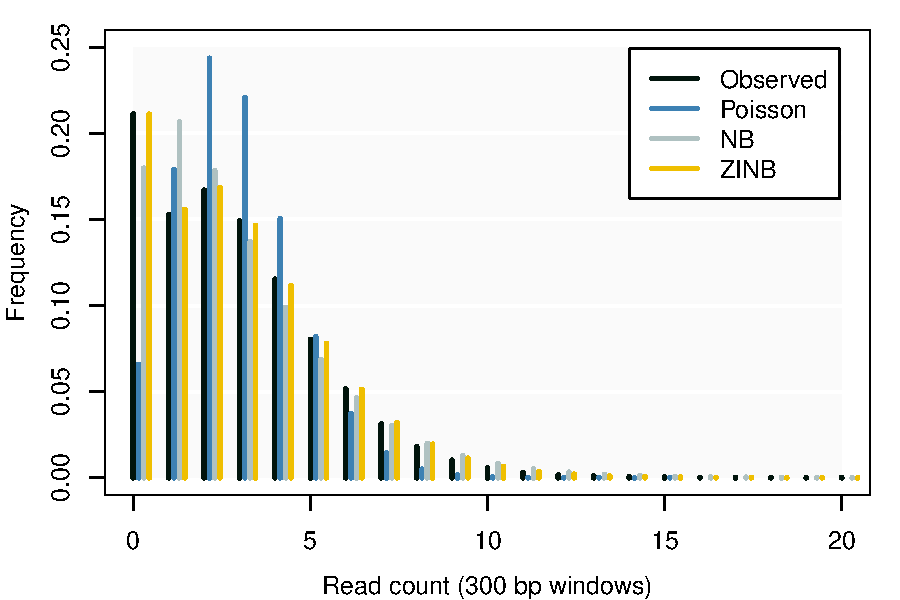
\includegraphics[scale=0.55]{ZINB_fit.pdf}}
% XX is wgEncodeSydhTfbsK562InputRawData.bed.gz %
\caption{Using the ZINB distribution to model ChIP-seq data. Reads from
the negative control dataset XX were mapped on the human genome and pooled
in 300~bp windows after removing duplicates. The histogram of the read
counts is shown in black (no immunoprecipitation was performed in this
experiment, so this variation corresponds to the `baseline'). The
histograms in gray scales show the maximum likelihood fit of the Poisson,
Negative Binomial (NB) and Zero-Inflated Negative Binomial (ZINB)
distributions. The fit of the Poisson distribution (light gray) is poor.
The NB distribution (medium gray) gives a good fit at the tail, but not
for windows with 0 and 1 read. The ZINB distribution (dark gray) gives
a good fit over the whole range.
}\label{fig:ZINB_fit}
\end{figure}

The NB distribution can be interpreted as a Gamma-Poisson process,
which gives a straightforward extension to a multivariate
distribution called the Negative Multinomial (NM) and to its
corresponding zero-inflated version the Zero-Inflated Negative
Multinomial (ZINM, see supplementary material for detail). In this model,
windows have an intrinsic ChIP-seq bias due to their sequence composition,
mappability and other inherent properties, which gives a baseline
variation present in all ChIP-seq experiments performed in the same
conditions. All the replicates of a ChIP-seq experiment can thus be
combined with the negative controls in a single multivariate
distribution.

\subsection{Discretization}
Discretization is performed by fitting an HMM
with ZINM emissions (see section \ref{sub:emissions}). The HMM has three
states corresponding to ``low'', ``medium'' and ``high'' abundance of
the given chromatin feature. We have observed that in many ChIP-seq
profiles, the baseline signal shows block-wise variations of low amplitude
but large size (typically 10-100 Kb). This will sometimes be the dominant
signal and a two-state HMM will identify these blocks instead of the
targets. Dedicating two states to fit the baseline is a way to make sure
that the ``high'' state corresponds to the targets of the chromatin
feature.

Fitting is performed with the Baum-Welch algorithm \citep{baum1966},
which is a special case of EM algorithm \citep{Dempster77maximumlikelihood}.
Discrete variables take only a small number of distinct values, which
allows to save computation time by hashing the observations. With this
technique, we need to compute each value of the emission probabilities
only once per cycle of the Baum-Welch algorithm. Transition parameters
are updated through the forward-backward algorithm, and emission
parameters are updated by solving maximum likelihood equations directly
with the Newton-Raphson method (see supplementary material for detail).
Approximately 3/4 of the computation time is spent in foward-backward
cycles, and 1/4 in updating emission parameters (the time spent computing
emission probabilities is insignificant). The algorithm stops when
parameters reach a stable value, or after a limit number of cycles (100
by default). The state calls are computed by finding the most likely
segmentation given the value of the parameters through the Viterbi
algorithm \citep{1054010}.

The shape parameter and the mixture ratio of the ZINM distribution
are fitted directly from the negative control profiles and they are
considered constant throughout. Overall, the total number of estimated
parameters is $3(r+1)$, where $r$ is the number of replicate experiments
(excluding negative controls).

\subsection{Classification and training}
\label{sub:training}
We used a machine learning strategy to identify discretization
failures. We first prepared a high confidence dataset where the
output of Zerone was labelled positive (success) or negative (failure).
We discretized 144 replicated ChIP-seq experiments (\textit{i.e.}
144 different features), together with their respective input control.
We labelled the output for the discretization as positive (91 cases)
or negative (53 cases), based visual inspection and on the available
literature about the chromatin features. The most common cases of
poor data quality in ChIP-seq correspond to low signal-to-noise ratio
(\textit{e.g.} when the antibody is unspecific), and lack of
repdroducibility between replicates (\textit{e.g.} when samples are
swapped). To cover these cases, we included in the trusted set
a number of cases obtained by discretizing non-replicates
(\textit{e.g.} CTCF and Pol2) and controls without
immuno-precipitation.
%% NOTE: there were a total of 802 non-replicate and flat discretizations

To identify discretization failures, we used the paremeters of the
fitted HMM. Based on the transition matrix, the emission paramaters,
the Viterbi Path and the posterior probabilities,
we computed 19 features expected to vary with the quality
of the discretization, and we used them to train a classifier.

Our first attempts with logistic regression suggested that linear
classifiers are unable to properly separate these two classes because
they overlap in the feature space (Fig.~\ref{fig:pca}). To obtain more
complex, nonlinear separation, we used a Support Vector Machine
(SVM, \cite{Chang2011,e1071}), as this approach guarantees the lowest
overfitting upper bound and allows nonlinear classification by mapping
the training data to a kernel space. Also, SVMs are fast to train and
they require only one hyperparameter to be fitted, which were
advantages over other approaches such as neural networks.

\begin{figure}[!tpb]
\centerline{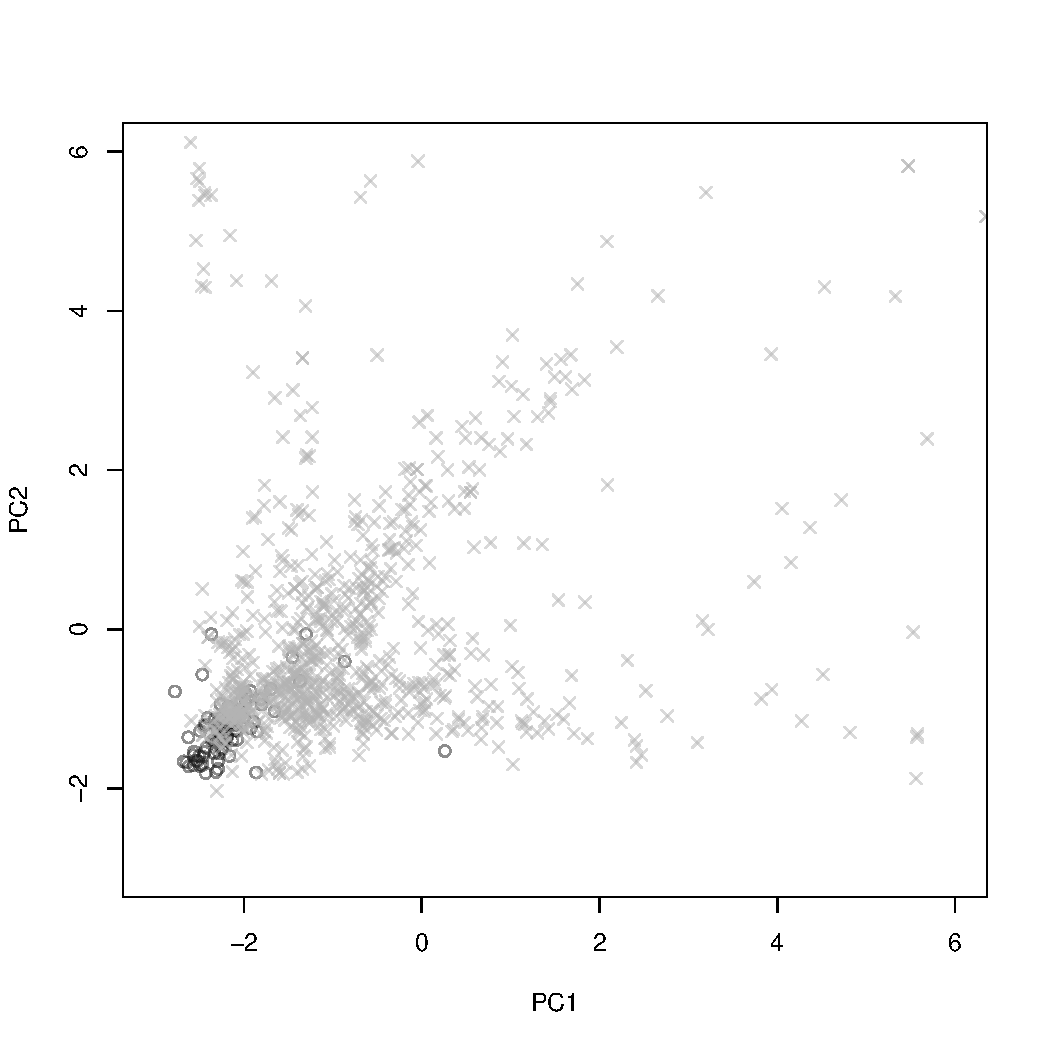
\includegraphics[scale=0.5]{pca.pdf}}
\caption{Principal Component Analysis of the training dataset.
Training examples labeled as positive (dark circles) appear to be similar to
each other, while negative examples (light crosses) show notable differences
between them and with respect to positive examples. There exist though a
certain degree of overlap between the two groups that creates an
``ambiguous zone'', at least in this projection.
}\label{fig:pca}
\end{figure}

We trained the SVM with a radial basis function kernel and
selected the hyperparameters that maximized the prediction
performance on test sets using a 10-fold cross-validation scheme.
The prediction accuracy on the trusted set was 95\%.
We then implemented a prediction function in Zerone that used the
model trained by the SVM to classify the discretizations and
suggest whether they should be accepted or discarded.

\subsection{Datasets and preprocessing}
We used all the ChIP-seq profiles produced by the ENCODE consortium
on the human myelogenous leukemia cell line K562. We did not make use
of preprocessed mapped reads because they could have been mapped with
different software and could therefore disagree on its results
\citep{pmid21059603}. Instead, we mapped all the raw reads onto the
hg19 assembly of the human genome with GEM \citep{pmid23103880}, using
the options \texttt{--unique-mapping} and \texttt{-q ignore} of gem-mapper,
version 1.376 (beta). The version of gem-indexer was 1.423 (beta). We
preprocessed the data in the same way both for training the classifier
and for benchmarking. We also used the same genome assembly to generate
the datasets used in the benchmarks (see Section \ref{sec:results}).

For training the classifier, we binned the mapped reads into 300~bp
windows and saved the data in WIG format before discretization.

\subsection{Benchmark conditions}
To compare Zerone to other discretizers, we analysed three different
ChIP-seq datasets: CCCTC-binding factor (CTCF), tri-methylated histone H3 at
lysine 36 (H3K36me3) and RNA polymerase II (Pol2)---that represent punctate,
broad and mixed type signals respectively. Each dataset consisted of an input
profile and two replicate target profiles.

To make the comparisons fair, we merged all contiguous windows that were called
as enriched by Zerone, in the same way the other programs do. Otherwise, the
number of enriched regions in the genome would be higher and Zerone performance
would look poorer than the actual.

We decided to include MACS \texttt{callpeak} (version 2.1.0.20140616) in
the comparisons because it is the \textit{de facto} standard method
for ChIP-seq peak calling; BayesPeak (version 1.20.0) because, as Zerone,
it makes use of an HMM with ZINB emissions to estimate the regions of
enrichment; and JAMM (version 1.0.7rev1) because it can perform joint
analysis on experimental replicates.

All tests were performed on an 8-core Intel Xeon E5606 machine with 48~GB of
DDR3-RAM at 1333~MHz. All programs were run on a single core with the default
options.

\end{methods}

\section{Results}
\label{sec:results}

% give an EXAMPLE where using Zerone highlighted inconsistencies in published
% ChIP-seq ENCODE data, allowing us to detect noisy and non-replicating profiles
% that should be flagged as such.

\subsection{Speed and memory consumption}
We compared the running time of the different programs on discretizing three
similar sized datasets that represent the three major types of ChIP-seq signal
usually observed. In our tests Zerone was the fastest algorithm, being a few
orders of magnitude faster than BayesPeak and JAMM, and a few times faster than
MACS (Fig.~\ref{fig:perf}, top row). This makes Zerone suitable for usage in
large volume pipelines. All programs behaved in a similar way on all three
datasets in terms of running time.

In terms of memory footprint, both Zerone and MACS were comparable, while
BayesPeak and JAMM demanded a few times times more memory (Fig.~\ref{fig:perf},
bottom row).

\begin{figure}[!tpb]
\centerline{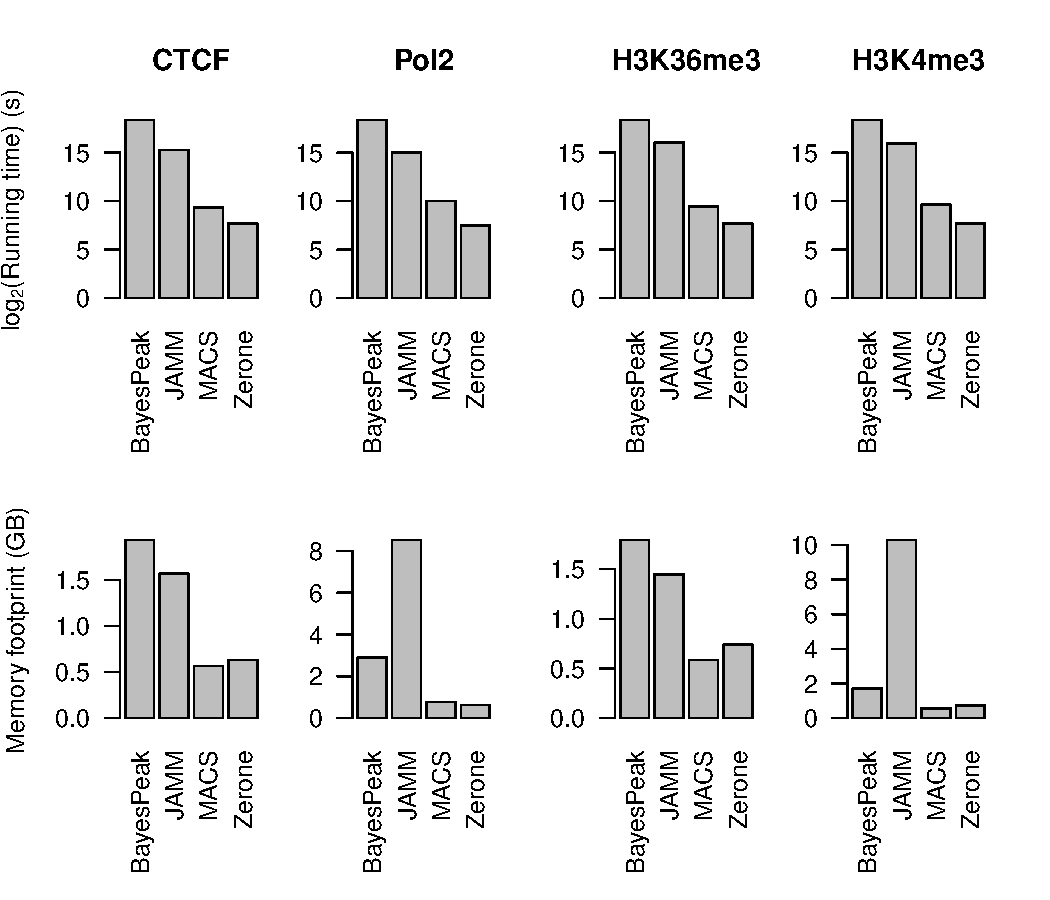
\includegraphics[scale=0.5]{performance.pdf}}
\caption{Running times and memory footprint of the different discretizers
on the three ChIP-seq datasets.
For programs that only allow single-profile discretization
(\textit{i.e.} BayesPeak and MACS), mean values are shown.
Note the logarithmic scale in the running times.
}\label{fig:perf}
\end{figure}

\subsection{Discretization benchmark}
There is currently no gold standard for benchmarking ChIP-seq discretizers
ability to call biologically relevant regions of enrichment. Therefore, we used
different strategies for comparing the different types of signals analyzed.

\subsubsection{Identification of CTCF binding sites.}
CTCF binding sites are characterized by a specific 20~bp sequence that is
highly conserved in vertebrates. In humans, nearly 80\% of these sites contain
the consensus motif \citep{pmid17382889}.
In order to determine the capacity of the different programs to call peaks of
CTCF binding, we compared the discretized profiles against a dataset of CTCF
binding motifs. We used FIMO \citep{pmid21330290} (MEME suite version 4.10.1,
\citealp{pmid19458158}) to generate such dataset from the human CTCF motif
obtained from the JASPAR database (version 5.0{\textunderscore}ALPHA,
\citealp{pmid24194598}). The CTCF motif dataset contained 85,690 entries.

Table \ref{tab:ctcf} shows that Zerone outperforms its competitors: it has one
of the highest recall scores, comparable to that of JAMM, the other software
capable of combined analysis, while achieving the highest precision among the
evaluated programs.

\begin{table}[!t]
\processtable{Summary of peak calling on the CTCF dataset.
The table lists the total number of peaks found by the different
programs, how many of those peaks contained at least one CTCF motif, and the
correspondent precision, recall and $F_{1}$ score relative to the CTCF motif
dataset.
\label{tab:ctcf}}
{\begin{tabular}{lrrccc}
        \toprule
        \textbf{Software}  & \textbf{Total}  & \textbf{Motif} &
        \textbf{Precision} & \textbf{Recall} & \textbf{$F_{1}$ score} \\
        \midrule
        BayesPeak$^{(1)}$ &  45,316 & 25,228 & 0.56 & 0.29 & 0.39 \\
        BayesPeak$^{(2)}$ &  45,154 & 23,428 & 0.52 & 0.27 & 0.36 \\
        JAMM              & 264,410 & 31,709 & 0.12 & 0.37 & 0.18 \\
        MACS$^{(1)}$      &  48,358 & 26,449 & 0.55 & 0.31 & 0.39 \\
        MACS$^{(2)}$      &  41,030 & 23,542 & 0.57 & 0.27 & 0.37 \\
        Zerone            &  50,792 & 30,972 & 0.61 & 0.36 & 0.45 \\
        \botrule
\end{tabular}}{
The numbers in parentheses indicate the results on the two replicates
by separate.}
\end{table}

\subsubsection{H3K36me3-enriched domains.}


\begin{figure}[!tpb]
    \centerline{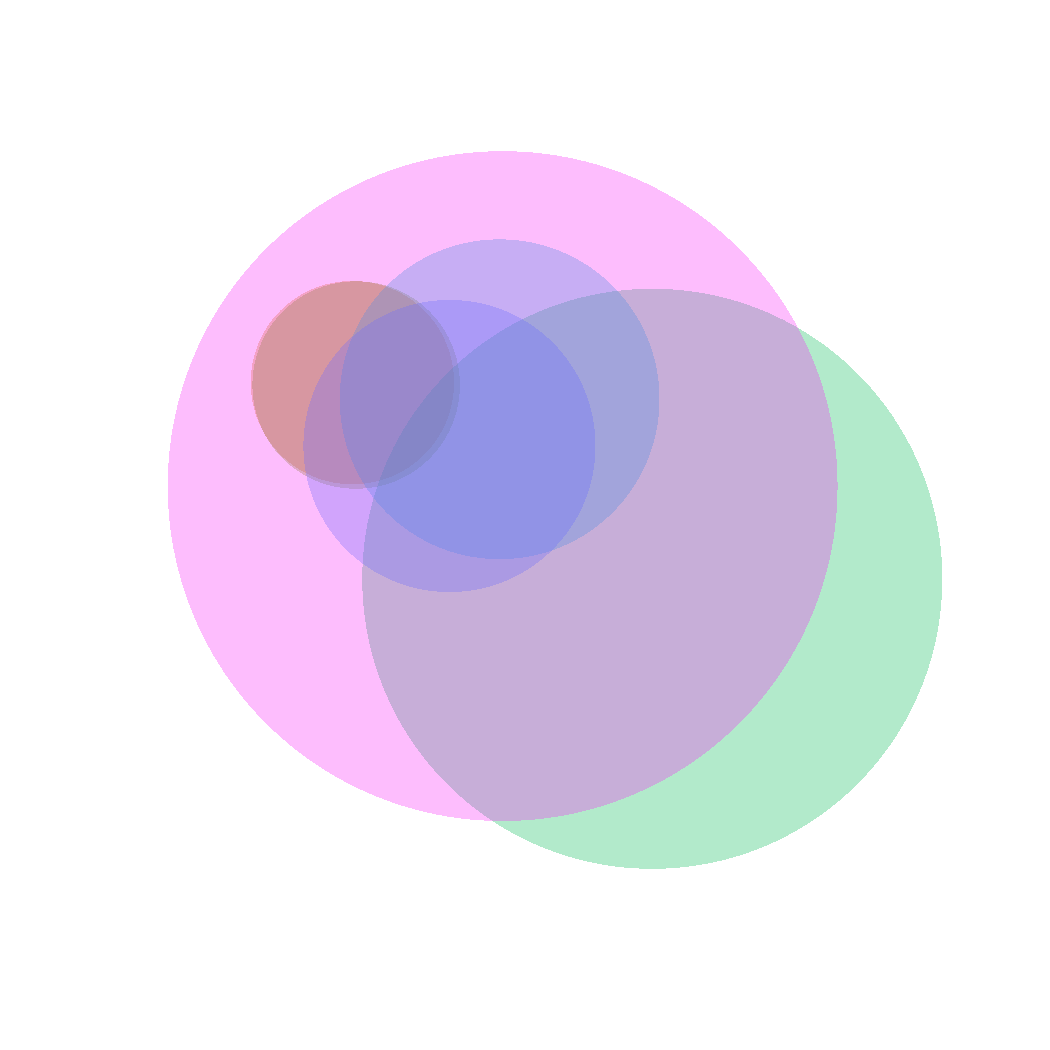
\includegraphics[scale=0.5]{histone_venn_color.pdf}}
\caption{Caption, caption.}\label{fig:venn}
\end{figure}

\subsubsection{Pol2 binding around transcription start sites.}
Pol2 profiles illustrate a characteristic binding pattern composed by a peaky
signal part near the transcription start site (TSS) and a broad type part
downstream of it \citep{pmid}. This represents the frequencies
at which Pol2 is poised or actively transcribing, respectively,
in the cell population \citep{pmid}.

To compare the behavior of the different discretizers, we determined how the
peaks were distributed around TSSs.

% figure: distance to tss (histogram or just % within a range??)
% with genomicranges distancetonearest cite

% TODO: implement BIN_SIZE as an option (default=300).
% RESULTS: Performance on test sets (around 95% on 10-fold cross-validation)

\section{Discussion and conclusion}
Some more text here.

\section*{Acknowledgement}

\paragraph{Funding\textcolon}
P.C. fellowship is partly financed by the Spanish Ministry of Economy and
Competitiveness (State Training Subprogram: predoctoral fellowships for the
training of PhD students (FPI) 2013).

\bibliographystyle{natbib}
\bibliography{document,extra}

\end{document}

%\begin{equation}
%\label{eq:01}
%\sum x+ y =Z
%\end{equation}

%\begin{enumerate}
%\item this is item, use enumerate
%\item this is item, use enumerate
%\item this is item, use enumerate
%\end{enumerate}

%\begin{itemize}
%\item for bulleted list, use itemize
%\item for bulleted list, use itemize
%\item for bulleted list, use itemize
%\end{itemize}

%\begin{table}[!t]
%\processtable{This is table caption\label{Tab:01}}
%{\begin{tabular}{llll}\toprule
%head1 & head2 & head3 & head4\\\midrule
%row1 & row1 & row1 & row1\\
%row2 & row2 & row2 & row2\\
%row3 & row3 & row3 & row3\\
%row4 & row4 & row4 & row4\\\botrule
%\end{tabular}}{This is a footnote}
%\end{table}

%\begin{figure}[!tpb]
%%\centerline{\includegraphics{fig01.eps}}
%\caption{Caption, caption.}\label{fig:01}
%\end{figure}
